\chapter{Branching and Multipass}
\label{c:branch.multi}

\index{branch}
\index{multipass}
The previous chapter (\sref{c:sequence}) covered how to construct a 
lattice branch using \vn{line}s and \vn{list}s. This chapter covers
how to connect the individual branches together to form an entire
accelerator complex. There are two ways this is done. To
describe a fork in an accelerator, \vn{branch} and \vn{photon_branch}
elements may be used. This is described in Section~\sref{s:branching}
With these elements, the connection between a transfer line and a
storage ring or the connection between a storage ring and an X-ray 
line can be simulated.

Branches may also share common elements such as the interaction region
shared by two storage rings. Here a \vn{multipass} line can be used
to describe this. Additionally, \vn{multipass} lines can be used
to describe the case where a beam goes through the same physical
element in a branch multiple times as in an energy recovery linac.
\vn{multipass} lines are described in Section~\sref{s:multipass}.

%-----------------------------------------------------------------------------
\section{Branching with Branch Elements}
\index{photon_branch}\index{branch}
\label{s:branching}

The root branches of a lattice are defined by the \vn{use}
(\sref{s:use}) statement. To further define such things as dump lines,
x-ray beam lines, transfer lines, etc., that branch off from a root
branch, a \vn{branch} or \vn{photon_branch} element (collectively they
can be called branching elements) is used.  \vn{Branch} elements can
define where the particle beam can branch off, say to a beam
dump. \vn{photon_branch} elements can define the source point for
X-ray beams.  Example:
\begin{example}
  erl: line = (..., dump, ...)               ! Define the root branch 
  use, erl
  dump: branch, to = d_line                  ! Define the branch point

  d_line: line = (..., q3d, ...)             ! Define the branch line
\end{example}
The difference between a \vn{branch} element and a \vn{photon_branch}
element is that for a \vn{branch} element the default particle for the
branch is the same as the line that the branch branches off from. The
default particle of the branch from a \vn{photon_branch} element is a
\vn{photon}. The actual particle associated with a branch can be set
by setting the \vn{particle} attribute of the branching element
(\sref{s:branch}).

\index{patch}
Branch lines can themselves have branching elements. A branch line always
starts out tangential to the line it is branching from. The
\vn{direction} attribute of the branch element indicates whether the
branch line is outgoing in the forward direction (direction = +1) or
incoming (direction = -1). A \vn{patch} element (\sref{s:patch}) can
be used at the beginning of a branch line to reorient the reference
orbit as needed.

Like the root branch \bmad always automatically creates an element
with \vn{element index} 0 at the beginning of each branch called
\vn{beginning}. The longitudinal \vn{s} position of an element in a
branch is determined by the distance from the beginning of the branch.

Branch parameters, like whether the branch is open
(``open'') or closed (``closed''), can be set
by setting the appropriate attribute of the \vn{branch} or
\vn{photon_branch} element used to orient the branch.
See \sref{s:branch} for more details.

Branches are named after the branching element name. In the above
example, the branch line would be named \vn{DUMP}. The root branch, by
default, is called after the name in the \vn{use} statement
(\sref{s:use}).

For branch lines (\sref{s:branching}), the ``branch
qualified'' name of an element is of the form
\begin{example}
  branch_name>>element_name
\end{example}
where \vn{branch_name} is the name of the branch and \vn{element_name} is the
``regular'' name of the element. Example:
\begin{example}
  root>>q10w
  xline>>cryst3
\end{example}
When parsing a lattice
file, branches are not formed until the lattice is expanded
(\sref{s:expand}). Therefore an \vn{expand_lattice} statement is
required before branch qualified names can be used in statements. 
See \sref{s:ele.names} for more details.

%-----------------------------------------------------------------------------
\section{Multipass}
\label{s:multipass}
\index{multipass|hyperbf}

Some lattices have the beam recirculating through the same element
multiple times. For example, an Energy Recovery Linac (ERL) will
circulate the beam back through the LINAC part to retrieve the energy
in the beam. In \bmad this situation can simulated using the
\vn{multipass} attribute. A simple example shows how this works.
\index{expand_lattice}
\begin{example}
  RF1: lcavity
  linac_part: line[multipass] = (RF1, ...)
  my_line: line = (linac_part, ..., linac_part)
  use, my_line
  expand_lattice
  RF1\B2[dphi0] = 0.5
\end{example}
The tracking part of the lattice consists of two slave elements
\begin{example}
  RF1\B1, ..., RF1\B2, ...
\end{example}
Since the two elements are derived from a \vn{multipass} line they are
given unique names by adding a \vn{{\B}n} suffix. In addition there is
a lord element (that doesn't get tracked through) called \vn{RF1} in the
lord part of the lattice. Changes to attributes of the lord \vn{RF1}
element will be passed to the slave elements by \bmad's bookkeeping
routines. Assuming \vn{RF1\B1} is an accelerating cavity, to make
\vn{RF1\B2} a decelerating cavity the \vn{dphi0} attribute of
\vn{RF1\B2} is set to 0.5. This is the one attribute that \bmad's
bookkeeping routines will not touch when transferring attribute values
from \vn{RF1} to its slaves. Notice that the \vn{dphi0} attribute had to
be set after \vn{expand_lattice} (\sref{s:expand})
is used to expand the lattice since
\bmad does immediate evaluation and \vn{RF1\B2} does not exist before
the lattice is expanded.

Sublines of a multipass line are automatically multipass:
\begin{example}
  a_line: line = (...)
  m_line: line[multipass] = (..., a_line, ...)
\end{example}
In this example \vn{a_line} is implicitly multipass.

Multiple elements of the same name in a multipass line are considered 
physically distinct:
\begin{example}
  m_line: line[multipass] = (A, A, B)
  u_line: line = (m_line, m_line)
  use, u_line
\end{example}
In this example the tracking part of the lattice is
\begin{example}
  A\B1, A\B1, B\B1, A\B2, A\B2, B\B2
\end{example}
In the control section of the lattice there will be two multipass
lords called \vn{A} and one called \vn{B}. The first \vn{A} lord 
controls the 1\St and 4\Th elements in the tracking part of the lattice 
and the second \vn{A} lord controls the 2\Nd and 5\Th elements.

%-----------------------------------------------------------------------------
\subsection{The Reference Energy in a Multipass Line}
\label{s:ref.e.multi}

\index{lcavity}
\index{p0c}\index{e_tot}\index{n_ref_pass}
If there are \vn{lcavity} elements in the lattice then the reference
energy at a given element may differ from pass to pass. In this case,
the normalized strength (k1, kick, etc.) for magnetic and electric
elements will not be the same from pass to pass. To avoid an
ambiguity, all magnetic and electric elements that are used in a
multipass line must have their magnetic or electric field strength set
as the independent attribute (\sref{s:depend}), {\em or} a reference
energy (\sref{s:energy}) must be defined. A reference energy is
defined by setting \vn{e_tot} or \vn{p0c}, or by setting
\vn{n_ref_pass} as described below. The default is for \vn{n_ref_pass}
to be set to 1.

To set the reference energy, one (and only one) of the attributes
\vn{n_ref_pass}, \vn{e_tot} or \vn{p0c} needs to be
set. \vn{n_ref_pass} is an integer indicating which pass is used to
define the reference energy for the lord element. The default if
nothing is set, is for \vn{n_ref_pass} to be set to 1.  Note: If
\vn{ref_orbit} is set to \vn{match_global_coords}, or for any element
where the reference energy is not constant (like an \vn{lcavity}),
\vn{n_ref_pass} must be used and must be set to 1.

%-----------------------------------------------------------------------------
\section{Branching and Multipass Examples}

Below are several examples of how branching and multipass can be used
to describe complicated machine geometries.

%-----------------------------------------------------------------------------
\subsection{Example: Flexible Patch in an ERL}
\label{s:ex.erl}

Consider the case of an Energy Recovery Linac (ERL) where the beam
goes through the linac section of the ERL twice. Once to accelerate
the beam and once to decellerate and recover the energy from the
beam. The basic ERL lattice is then
\begin{example}
  erl: line = (injector, linac, arc, linac, dump)
  injector: line = (...)
  linac: line[multipass] = (..., rf1, ...)
  arc: line = (..., patch2)
  dump: line = (...)
  patch2: patch, flexible = True
  ...
  expand_lattice
  rf1\B2[dphi0] = 0.5
  ...
\end{example}

%-----------------------------------------------------------------------------
\subsection{Example: Injection Line Into a Dipole}
\label{s:ex.inj}

\begin{figure}[tb]
  \centering
  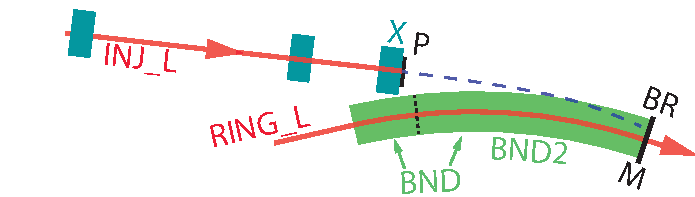
\includegraphics[width=5in]{injection.pdf}
  \caption[Injection line into a dipole magnet.]{Injection line into a dipole magnet.}
  \label{f:inject}
\end{figure}

An injection line into a dipole magnet is illustrated in \fig{f:inject}.



%-----------------------------------------------------------------------------
\subsection{Example: Colliding Beam Storage Rings}
\label{s:ex.collide}

\begin{figure}[tb]
  \centering
  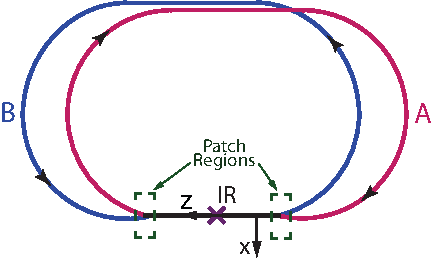
\includegraphics[width=5in]{colliding-beams.pdf}
  \caption[Dual ring colliding beam machine]{Dual ring colliding beam machine. 
The beam in the \vn{A} ring rotates clockwise and in the \vn{B} ring
counterclockwise.}
  \label{f:collide}
\end{figure}

The idealized layout of a pair of storage rings used for colliding
counter rotating beams is shown in \fig{f:collide}. Rings \vn{A} and
\vn{B} intersect at two interaction regions labeled \vn{ir1} and
\vn{ir2} where the beams collide. The basic lattice description is:
\begin{example}
  ir1: line[multipass] = (...)
  ir2: line[multipass] = (...)
  m: marker
  fid: fiducial, origin_ele = m
  ...
  a: line = (arc_a1, pa1_in, ir1, m, pa1_out, arc_a2, pa2_in, ir2, pa2_out)
  b_rev: line = (arc_b1, pb1_in, ir1, fid, pb1_out, arc_b2, pb2_in, ir2, pb2_out)
  b: line = (--b_rev)
  use, a, b
\end{example}
Lines \vn{ir1} and \vn{ir2} are the two interaction regions which are
declaired \vn{multipass} since they are shared by the two rings. Line
\vn{a} represents ring \vn{A} where the beam which, by definition,
travels in the same direction as increasing $s$, rotates clockwise.
Line \vn{b_rev} is a ``reversed'' line of ring \vn{B} and, like
\vn{a}, represents a beam rotating clockwise.  Line \vn{b}, which
represents ring \vn{B}, is the reverse of \vn{b_rev} and here the beam
rotates counterclockwise. In this construction, all elements of \vn{b}
are reversed.  While this is not manditory (only the interaction
regions must be reversed in \vn{b}), having all of \vn{b} reversed
simplifies the geometry since this means that the local coordinate
systems of both lines \vn{a} and \vn{b} will be ``aligned'' with the
$x$-axis pointing to the outside of the ring and the $y$-axis pointing
up, out of the page. Having non-aligned coordinate systems is possible
but potentially very confusing.

The two rings are physically aligned using a marker \vn{m} in \vn{a}
and a \vn{fiducial} element \vn{fid} in \vn{b} that aligns with
\vn{m}.  Each ring has four rigid \vn{patch} elements, whose name
begins with \vn{p}, on either side of each interaction region.

The finished lattice will have two branches, The first branch (with
index 0) will be derived from line \vn{a} and the second branch (with
index 1) will be derived from line \vn{b}. The multipass lords
representing the physical IR elements will be in the ``lord section''
of branch 0. 
